\chapter{Introducción} \label{ch:introduccion}

Este proyecto es software libre, y está liberado con la licencia \cite{agplv3}.

\section{Motivación}

Vivimos en tiempos extraños, desde diciembre de 2019 escuchamos hablar sobre la aparición de un brote epidemiológico de neumonía cuya causa era desconocida por aquel entonces en la ciudad china de Wuhan. Este brote tuvo lugar en el mercado de la ciudad y tras el aviso de las autoridades competentes de Wuhan a la OMS (Organización Mundial de la Salud) se empezó a investigar que podría estar provocando dicho brote. Esto hizo que tras varias investigaciones se conociera que la causa del mismo era la aparición de un nuevo coronavirus \cite{oms-covid} de tipo zoonótico; al cual se le dio el nombre de Covid-19. Según declaraciones de la OMS, este virus presentaba un riesgo para la salud pública, bajo las regulaciones del Reglamento Sanitario Internacional \cite{reglamento-sanitario-internacional} y posteriormente este sería considerado como una pandemia.

Poco a poco este nuevo virus fue extendiéndose, empezando por el continente asiático y por el resto del planeta.Todos y cada uno de los países afectados han aportado los datos de las diferentes incidencias que ha tenido el virus dentro de sus fronteras, aunque a pesar de ello seguimos sin conocer el alcance real de la pandemia ya que no existe un criterio común para la publicación de los datos, si no que cada país los calcula siguiendo los métodos que considera oportunos, por lo que la incidencia puede ser incluso mayor de lo mostrado por los datos, pero no vamos a centrarnos en como se calculan dichos datos.

Basándonos en esto, sabemos que existe una preocupación por parte de la población hacia el virus, a la cual le gusta estar informada. Hoy en día es importante estar bien informado, como nos muestra Gabriela Nova en su articulo "Los beneficios de estar informado" \cite{gabriela-nova}. Por ello, la mayor preocupación de la gente es conocer información a cerca del virus, de como está evolucionando, cuantas contagios, muertes y altas se han producido, entre otros datos. Podemos comprobar que actualmente el Covid-19 es una de las principales preocupaciones de la población, algunas de ellas que aparecen como consecuencia del propio virus. La Figura \ref{fig:preocupaciones} refleja una tabla con las preocupaciones principales de la población, donde se puede apreciar que el Covid-19 es la segunda preocupación de los españoles.

\begin{figure}[htb]
	\centering
	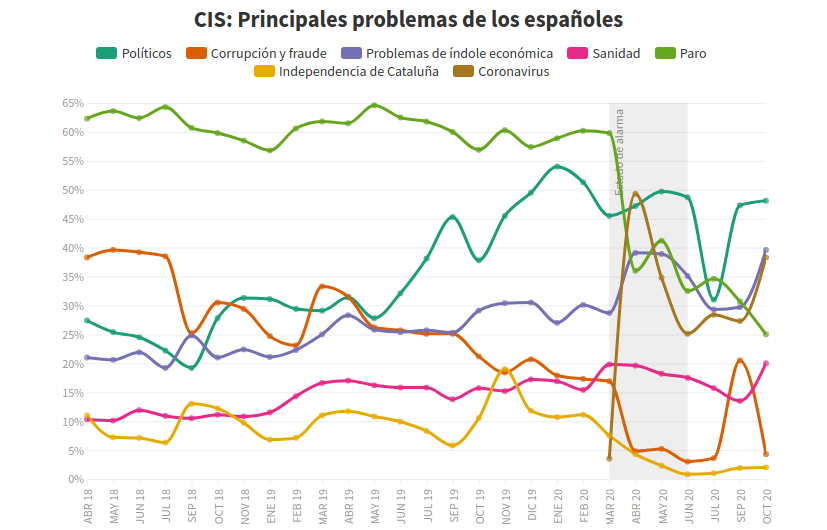
\includegraphics[width=1\textwidth]{img/preocupaciones}
	\caption{Preocupaciones de la población española. Fuente: \cite{rtve-preocupaciones}}
	\label{fig:preocupaciones}
\end{figure}

Como hemos dicho, a la gente le gusta estar informada, y más ahora, por lo que la transparencia en una situación como la que se está viviendo es algo más que esencial. Esta información tiene como funcionalidad mantener a la gente tranquila, pudiendo aportarles datos de la evolución de la pandemia, pero no solo eso, si no que también sirven para hacer un análisis de cara a la implementación y toma de medidas por parte de los gobiernos de los países afectados. Sin embargo todos estos datos a pesar de ser accesibles para la población, presentan un problema, la difícil visualización de esto de una manera sencilla e intuitiva. En este punto podemos hacernos una pregunta: ¿como podemos ofrecer esa información de manera que pueda ser útil a toda la población que quiera consultar y hacer uso de ella?

La respuesta a la pregunta anterior podemos decir que puede llegar a ser obvia en los tiempos en los que vivimos, donde la tecnología se ha instalado para quedarse en nuestra vida, por lo que podríamos decir que la respuesta a nuestra pregunta es: hacer uso de la tecnología. Los smartphones es un producto que hoy en día todo el mundo tiene, según la web Stadista \cite{statista}, en 2019 alrededor de los 2.650 millones de usuarios cuentan con uno. Para ser mas concretos el 96\% de los ciudadanos españoles mayores de 14 años que acceden a internet lo hacen desde su smartphone. De la misma forma un 92\% usa el móvil todos los días en una media de 3 horas diarias según el siguiente artículo \cite{elperiodico}.

\section{Alcance}

Este proyecto está pensado para poder llegar a una gran número de usuarios de todo el país. Lo que se pretende es que sean los propios usuarios los encargados de dar a conocer el proyecto. Sabemos que a veces el propio boca a boca es una de las maneras más eficaces de propagación, y en la época en la que nos situamos las personas suelen buscar recomendaciones sobre los productos que van a consumir o utilizar. Si tu como usuario estas contento con la aplicación se la recomendarás a más gente de tu entorno, lo que provocará no solo un aumento de usuarios, ya que estos se lo dirán a su vez a otros, con el fin de conseguir llegar al máximo número de personas posibles, proporcionándole información sobre la enfermedad.

Como hemos mencionado al inicio, toda la información puede ser consultada por la propia población, ¿entonces que sentido tiene este proyecto?. Entre otras cosas, cada Comunidad Autonómica tiene su propia manera de publicar los datos, a veces de una manera más sencilla y otras de una manera más compleja. Por ello lo que se pretende con \textbf{Covid-19 Reports} es poder agrupar toda esta información en un mismo lugar, facilitando el acceso a los usuarios y mostrando información adicional, por ejemplo, gráficos de la evolución de los datos seleccionados.

\section{Objetivos generales}

El objetivo principal de este proyecto es el desarrollo de un bot móvil orientado a informar a la población española para poder conocer los datos más relevantes sobre la pandemia del Covid-19 de una manera fiable. Este nos permitirá la consulta, tanto a nivel de todo el país como de las diferentes Comunidades Autónomas, de datos como el incremento de los casos desde el inicio de la pandemia, los casos registrados las últimas 24 horas, el número de fallecidos, los datos hospitalarios, etc.

Para llevar a cabo el proyecto se pondrá en práctica la metodología de desarrollo Scrum, la cual usaremos para la planificación y desarrollo del proyecto, con el fin de aprovechar las ventajas que esta nos ofrece.

Está claro, como hemos dicho antes, que una de las mayores preocupaciones de la población es el Covid-19, Por ello, \textbf{Covid-19 Reports} se ha llevado a cabo con el fin de evitar una desinformación en cuanto a los datos y la evolución de esta pandemia se refieren, estando de forma libre y accesible para todos lo usuarios que así quieran hacer uso de ella.

También es cierto, que estos mismos datos ya pueden ser consultados en diferentes lugares, como son las webs de los propios organismos de gobiernos, pero también lo es que cada organismo adapta esos datos y su acceso según ellos crean convenientes y adaptándose a estructuras en sus webs que ya disponían. Por todo ello, otro de los objetivos de este bot es la de no solo unificar, si no la de mostrar de una forma sencilla e idéntica los datos, evitando tener que aprender a como acceder a los datos o evitar la confusión del usuario si desea consultar los datos de otra comunidad, bien por ver la evolución, o bien para conocer la situación en todas las Comunidades Autónomas del país.